\documentclass[titlepage]{article}
\usepackage{listings}
\usepackage[final]{pdfpages}

\lstset{%
  numbers=left,
  numberstyle=\tiny,
  basicstyle=\ttfamily,
  breaklines=true,
  frame=tb
}

\lstdefinestyle{CANSI}
{
    language=[Ansi]C,
    literate = *{\ \ }{}0, %replaces each occurence of two consecutive spaces by one
    columns=fullflexible,
    showstringspaces=false,
    keywordstyle=\color{black}
}

\lstdefinestyle{Token}
{
    breaklines=false,
    literate = *{\ \ \ \ \ \ \ }{}0, %replaces each occurence of two consecutive spaces by one
    columns=1
}

\setlength{\columnsep}{20pt}

\newcommand{\ShowSourceFile}[2]
{
% \begin{lstlisting}[breaklines]
%     \VerbatimInput[fontsize=\footnotesize{}, frame=lines,label=#2]{#1}
% \end{lstlisting}
    \lstinputlisting[style=CANSI, caption=#2]{#1}
}

\newcommand{\ShowSampleFile}[2]
{
% \begin{lstlisting}[breaklines]
%     \VerbatimInput[fontsize=\footnotesize{}, frame=lines,label=#2]{#1}
% \end{lstlisting}
    \lstinputlisting[caption=#2]{#1}
}

\newcommand{\ShowTokenFile}[2]
{
% \begin{lstlisting}[breaklines]
%     \VerbatimInput[fontsize=\footnotesize{}, frame=lines,label=#2]{#1}
% \end{lstlisting}
    \lstinputlisting[style=Token,caption=#2]{#1}
}
% \RecustomVerbatimCommand{\VerbatimInput}{VerbatimInput}%
% {
% fontsize=\footnotesize{},
%
%  frame=lines,  % top and bottom rule only
%  framesep=2em, % separation between frame and text
%  % rulecolor=\color{Gray},
%
%  % label=\fbox{\color{Black}data.txt},
%  labelposition=topline
% }

\author{Nate Beckemeyer}
\title{\textbf{CS 4013: Compiler Construction: Project 2}}
\date{December 2016}



\begin{document}
    \maketitle
    \section*{Introduction}
    % For Project 1, I wrote a lexical analyzer in C for Pascal. The purpose
    % of the lexical analyzer is to  break down the Pascal source code into
    % the parts needed to construct a parse tree. To achieve that goal, the
    % lexical analyzer identifies each lexeme in the code, such as the parts
    % of a type declaration, `:' and `integer' or `real', the beginning of a
    % program, `program', or perhaps the multiplication operator, `*'. It converts
    % this lexeme into a token that later parts of the compiler can readily use.
    %
    % The user can specify a source document for the analyzer, and the
    % analyzer will create a listing file and a token file. The listing file
    % contains the source program, line-by-line, but points out any lexical
    % errors that occur. The token file contains the line number, the lexeme
    % corresponding to the token, the type of the token, and the attribute
    % value of the token.
    For Project 2, I massaged the modified Pascal grammar into an $LL(1)$
    grammar. According to that grammar, I implemented a recursive descent parser
    to construct the parse tree.

    The compiler detects any lexical and syntax errors that occur, and reports
    them in the listing file.

    \section{Methodology}
    The recursive descent parser matches productions, starting with the
    ``program'' production. The productions are outlined in the grammars
    included below. The documents are in the following order:
    \begin{enumerate}
        \item The initial grammar without epsilon productions.
        \item The new grammar having eliminated left recursion.
        \item That grammar now left-factored to become an $LL(1)$ grammar.
        \item The first and follows sets for each production.
        \item The parse table.
    \end{enumerate}

    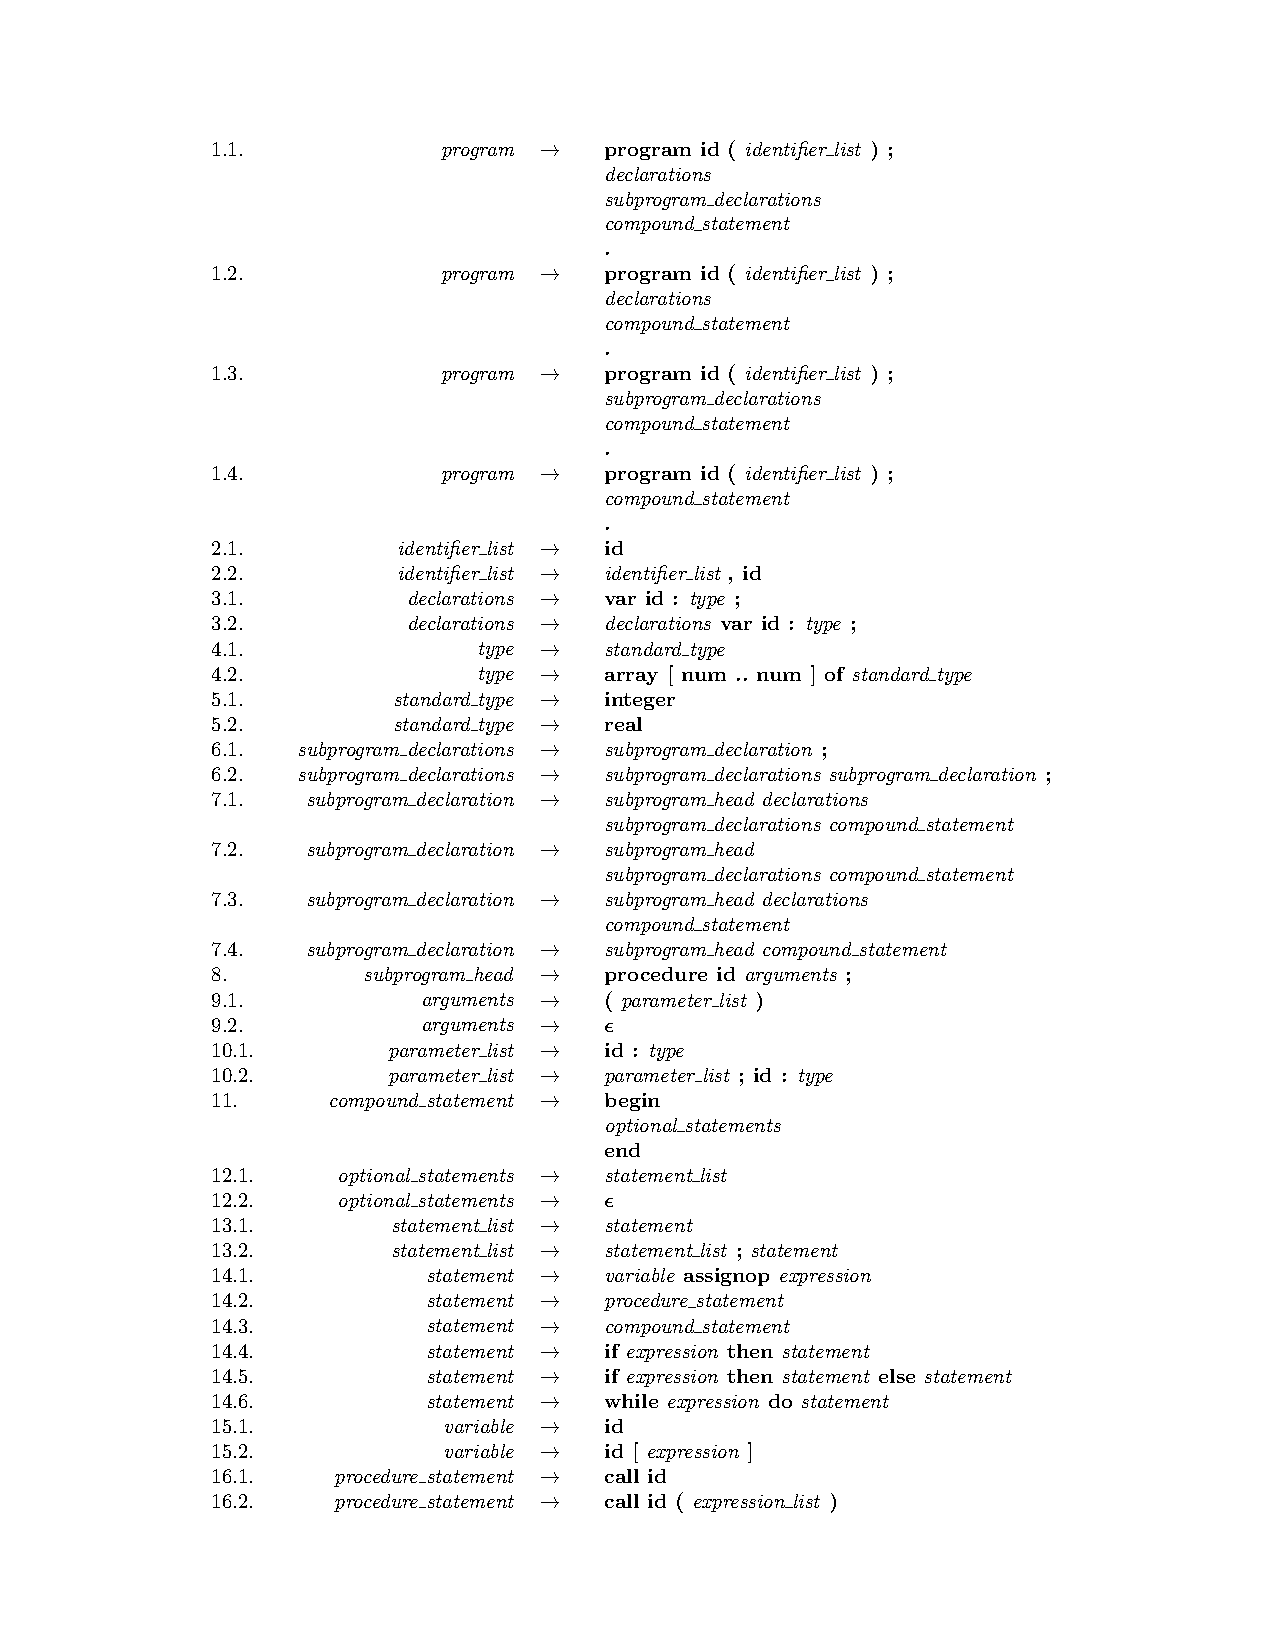
\includepdf[pages=-]{grammar_steps/sansEpsilon.pdf}
    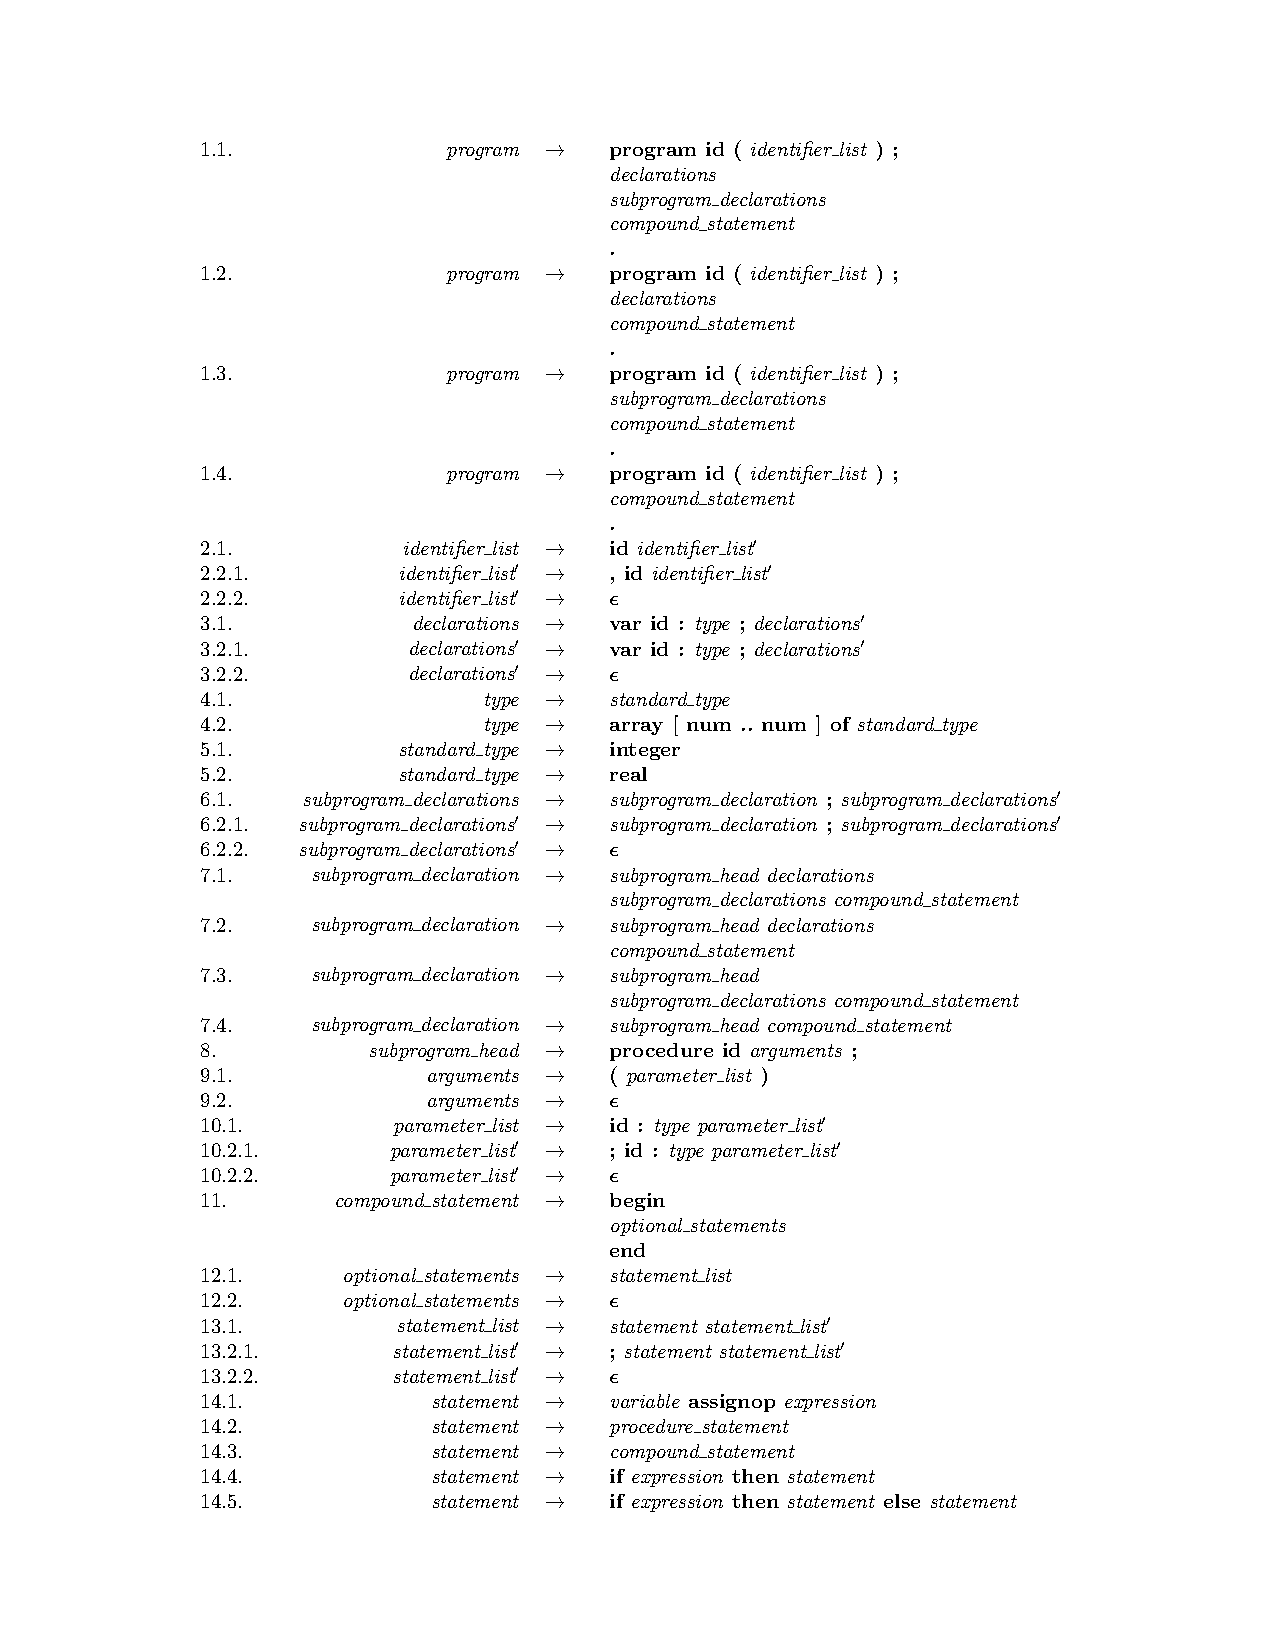
\includepdf[pages=-]{grammar_steps/sansLeftRecursion.pdf}
    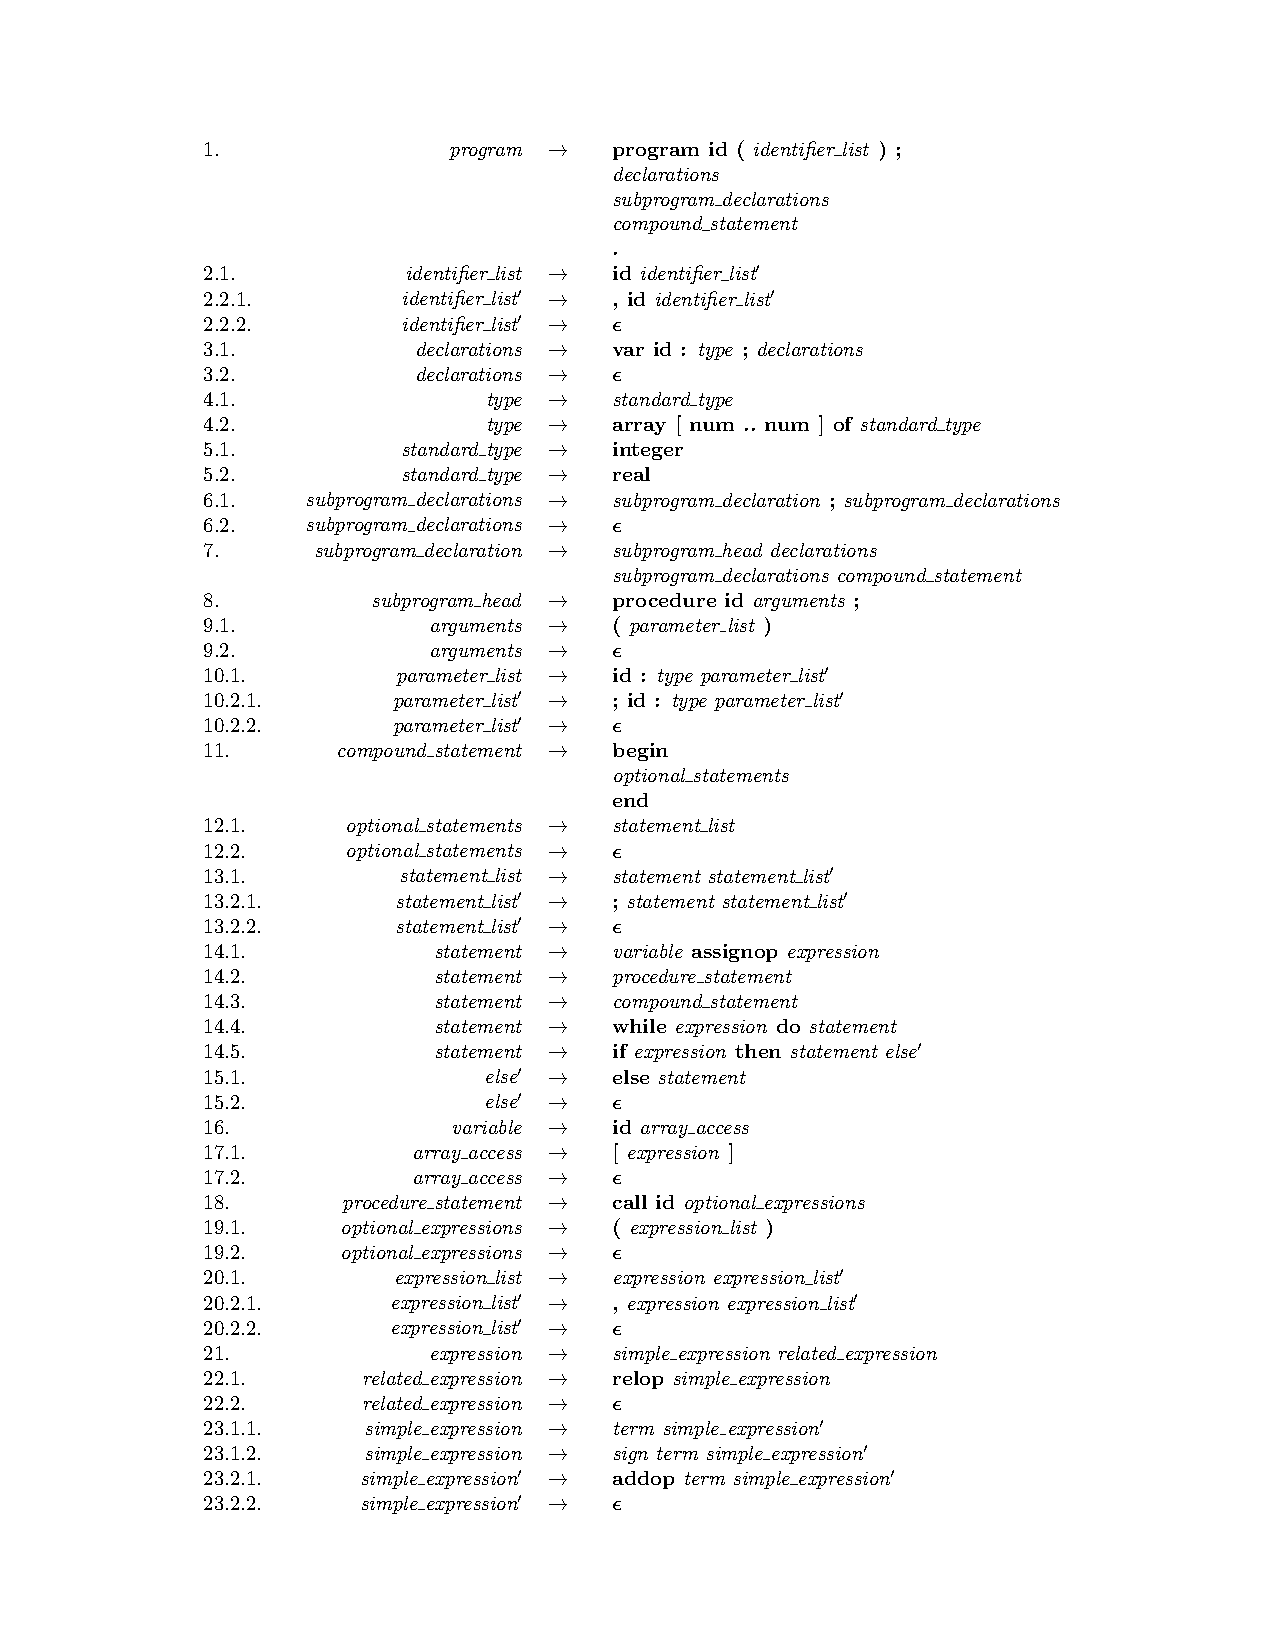
\includepdf[pages=-]{grammar_steps/leftFactored.pdf}
    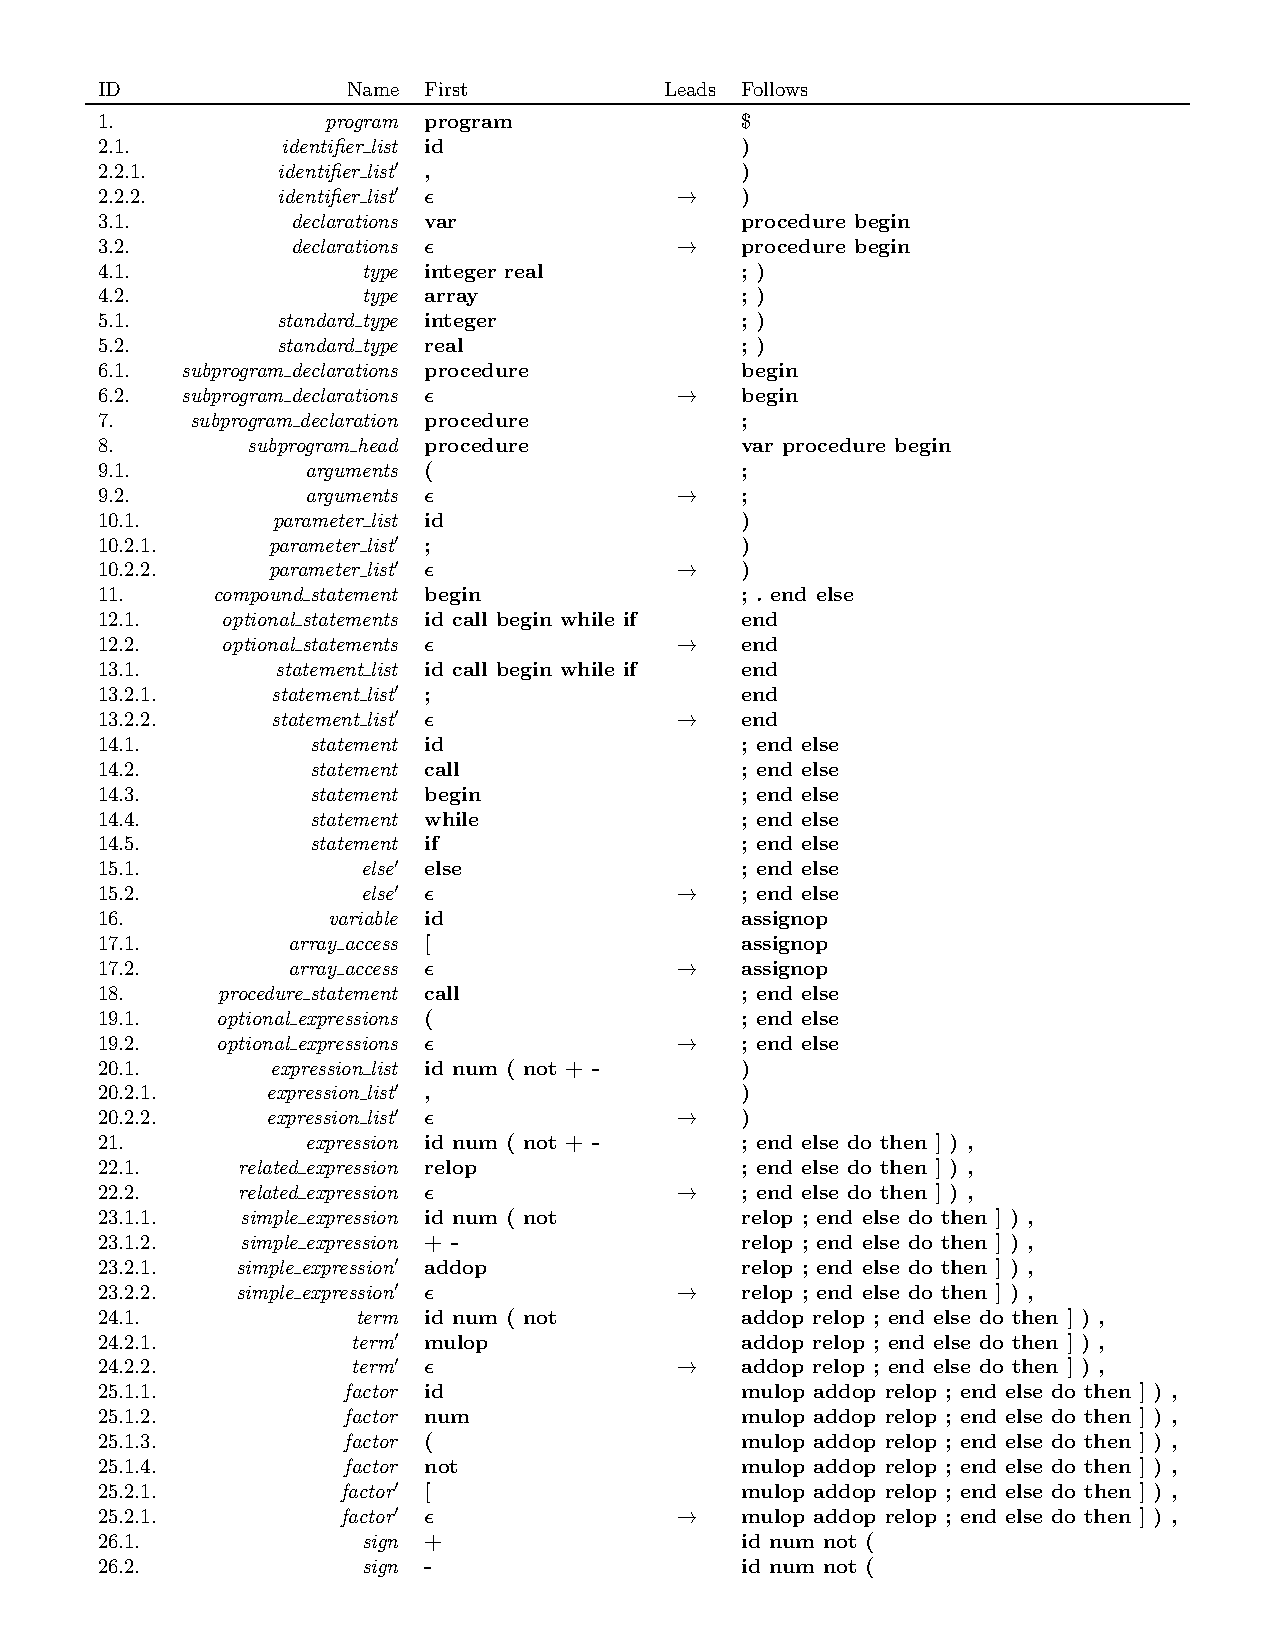
\includepdf[pages=-]{grammar_steps/firstAndFollows.pdf}
    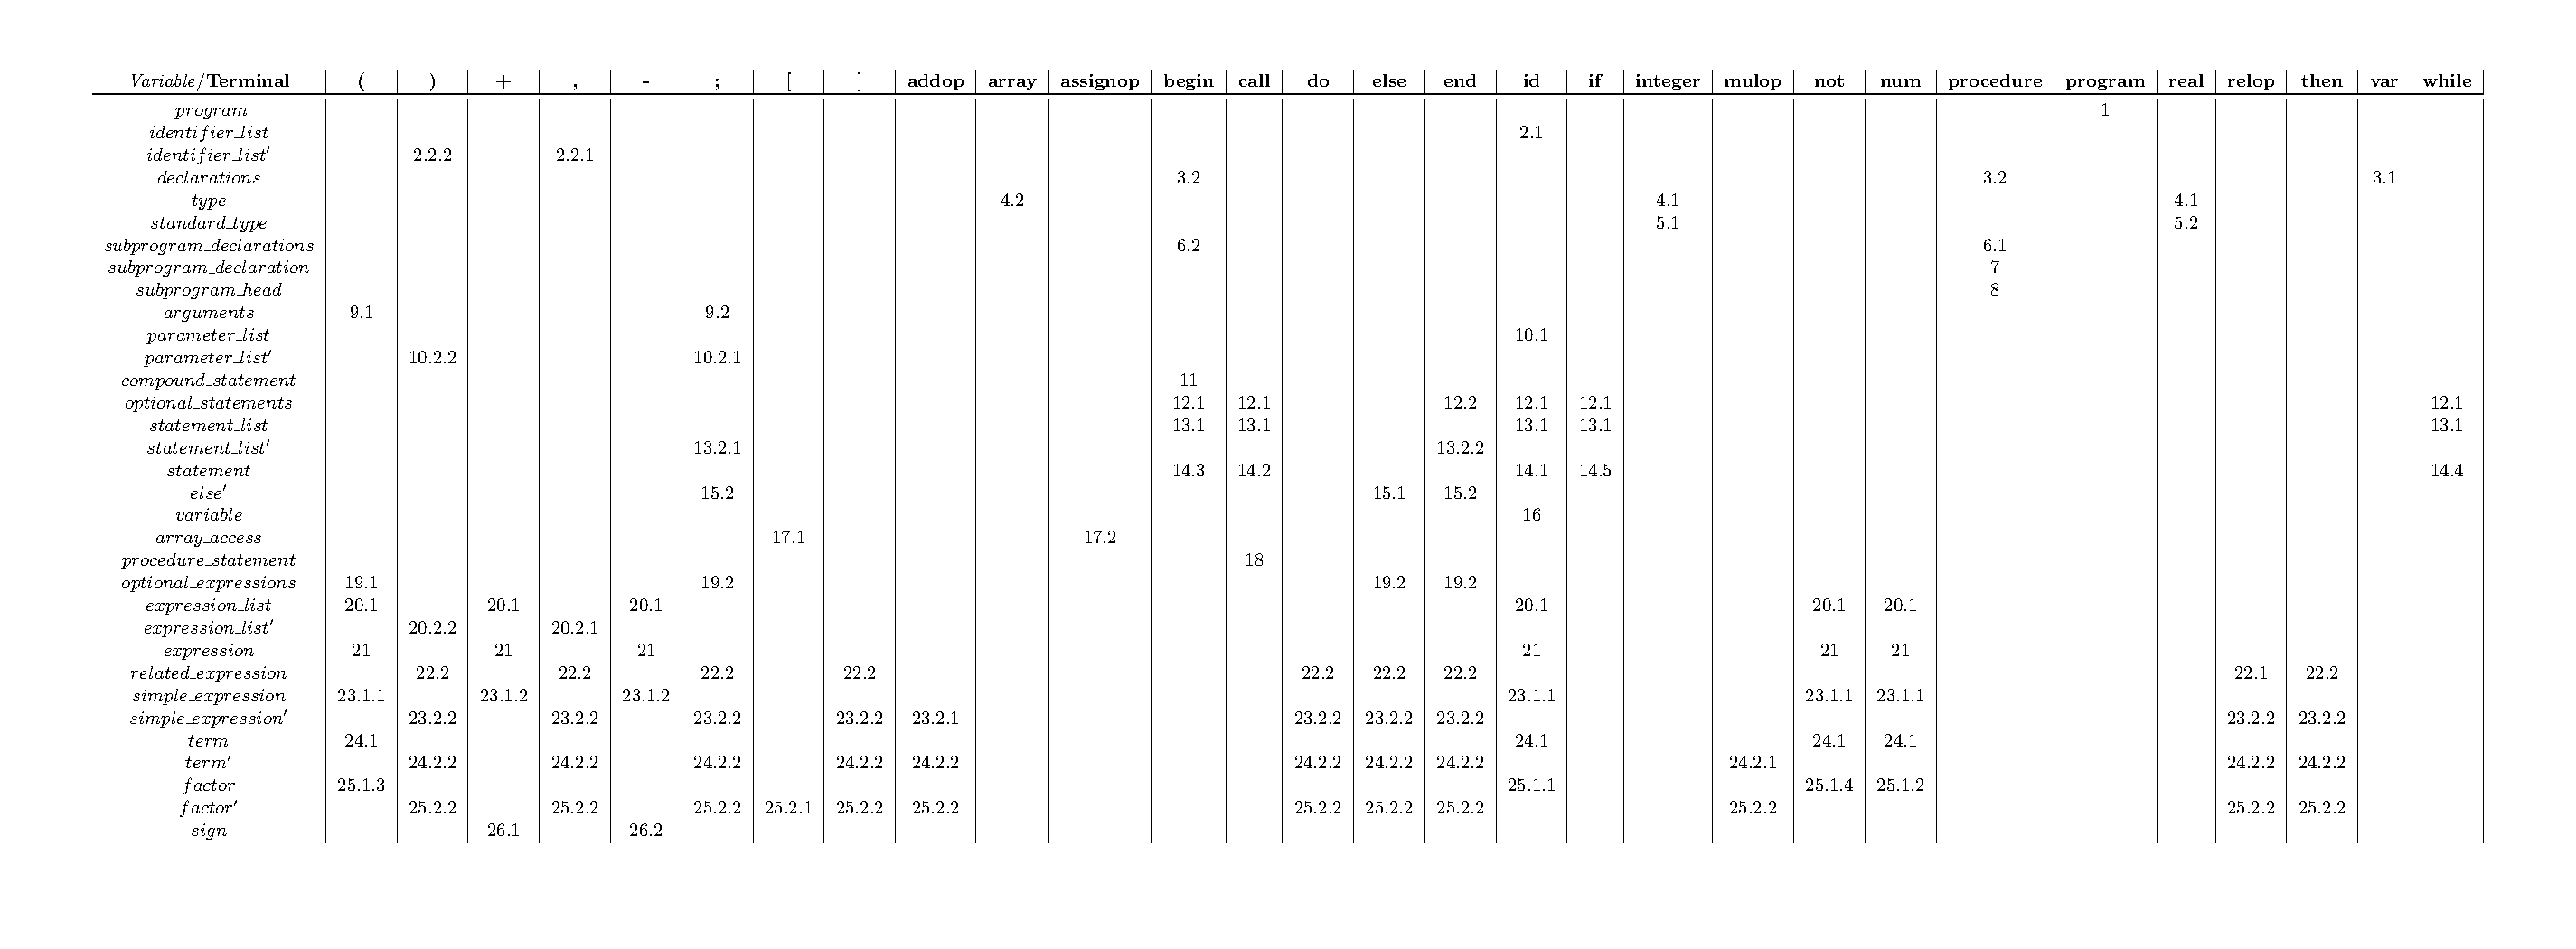
\includepdf[pages=-]{grammar_steps/parseTable.pdf}

    \section{Implementation}
    Each production resides in its own file, where it's first and synch sets
    are specified. The ``program'' production is called when the compiler
    begins, and it requests the next tokens. From there, productions are called
    in accordance to the grammar rules and the tokens receieved from the lexical
    analyzer.

    The ``match'' function matched the token and set a global variable named
    ``current\_tok'' to the next token. If the match failed, an syntax error
    was printed to the listing file. Another operation called
    ``require\_synch'' was included, in the event that no token could
    identify the current production in a grammar variable. $require\_synch$
    would take in the firsts and synch sets of the grammar variables, print the
    appropriate error message (``recieved X; expected Y, Z''), then discard %chktex 13
    tokens until an item from the synch set were matched.

    The productions mapped $1:1$ from terminal symbols to match and
    from grammar variables to productions. Which production to use
    in which grammar variable was determined by the value of $current\_tok$
    (hence the $LL(1)$ property of our grammar).

    If any errors were encountered while parsing, the error is added
    to the error queue. Then, the error is printed before the next token
    is collected.

    \section{Discussion \& Conclusions}
    Implementing this project definitely taught me about the importance
    of an $LL(1)$ grammar, and how neat the recursive descent parser is.
    I also noticed that the $require\_synch()$ function would have been
    wonderful as a dynamically-scoped function.

    I wrote this compiler in C, with no external code of any kind. It was
    compiled with clang on macOS Sierra.

    \clearpage{}
    \section*{Appendix 1: Sample Inputs and Outputs} % Input and output files.
    \subsection{Error-Filled Source File}
    \ShowSampleFile{appendix1/error_full/debug.pas}{Error-Full Source Code}
    \ShowSampleFile{appendix1/error_full/listing.txt}{Error-Full Listing File}
    \ShowTokenFile{appendix1/error_full/tokens.dat}{Error-Full Token File}

    \subsection{Error-Free Source File}
    \ShowSampleFile{appendix1/error_free/debug.pas}{Error-Free Source Code}
    \ShowSampleFile{appendix1/error_free/listing.txt}{Error-Free Listing File}
    \ShowTokenFile{appendix1/error_free/tokens.dat}{Error-Free Token File}

    \twocolumn{}
    \section*{Appendix 2: Program Listings}
    \ShowSourceFile{code/compiler.c}{compiler.c}
    \ShowSourceFile{code/dataStructures/declarationsTree/declarationsTree.h}{declarationsTree.h}
    \ShowSourceFile{code/dataStructures/linkedList/linkedlist.h}{linkedlist.h}
    \ShowSourceFile{code/errorHandler/errorHandler.h}{errorHandler.h}
    \ShowSourceFile{code/globals/globals.h}{globals.h}
    \ShowSourceFile{code/handler/handler.h}{handler.h}
    \ShowSourceFile{code/parser/parser.h}{parser.h}
    \ShowSourceFile{code/parser/productions/productions.h}{productions.h}
    \ShowSourceFile{code/symbolTable/symbolTable.h}{symbolTable.h}
    \ShowSourceFile{code/tokenizer/machines/machines.h}{machines.h}
    \ShowSourceFile{code/tokenizer/tokenizer.h}{tokenizer.h}
    \ShowSourceFile{code/tokenizer/tokens.h}{tokens.h}
    \ShowSourceFile{code/dataStructures/declarationsTree/declarationsTree.c}{declarationsTree.c}
    \ShowSourceFile{code/dataStructures/linkedList/linkedlist.c}{linkedlist.c}
    \ShowSourceFile{code/errorHandler/errorHandler.c}{errorHandler.c}
    \ShowSourceFile{code/globals/globals.c}{globals.c}
    \ShowSourceFile{code/handler/handler.c}{handler.c}
    \ShowSourceFile{code/parser/parser.c}{parser.c}
    \ShowSourceFile{code/parser/productions/arguments.c}{arguments.c}
    \ShowSourceFile{code/parser/productions/array_access.c}{array_access.c}
    \ShowSourceFile{code/parser/productions/compound_statement.c}{compound_statement.c}
    \ShowSourceFile{code/parser/productions/declarations.c}{declarations.c}
    \ShowSourceFile{code/parser/productions/else_tail.c}{else_tail.c}
    \ShowSourceFile{code/parser/productions/expression.c}{expression.c}
    \ShowSourceFile{code/parser/productions/expression_list.c}{expression_list.c}
    \ShowSourceFile{code/parser/productions/expression_list_tail.c}{expression_list_tail.c}
    \ShowSourceFile{code/parser/productions/factor.c}{factor.c}
    \ShowSourceFile{code/parser/productions/factor_tail.c}{factor_tail.c}
    \ShowSourceFile{code/parser/productions/id_list.c}{id_list.c}
    \ShowSourceFile{code/parser/productions/id_list_tail.c}{id_list_tail.c}
    \ShowSourceFile{code/parser/productions/optional_expressions.c}{optional_expressions.c}
    \ShowSourceFile{code/parser/productions/optional_statements.c}{optional_statements.c}
    \ShowSourceFile{code/parser/productions/parameter_list.c}{parameter_list.c}
    \ShowSourceFile{code/parser/productions/parameter_list_tail.c}{parameter_list_tail.c}
    \ShowSourceFile{code/parser/productions/procedure_statement.c}{procedure_statement.c}
    \ShowSourceFile{code/parser/productions/program.c}{program.c}
    \ShowSourceFile{code/parser/productions/related_expression.c}{related_expression.c}
    \ShowSourceFile{code/parser/productions/sign.c}{sign.c}
    \ShowSourceFile{code/parser/productions/simple_expression.c}{simple_expression.c}
    \ShowSourceFile{code/parser/productions/simple_expression_tail.c}{simple_expression_tail.c}
    \ShowSourceFile{code/parser/productions/standard_type.c}{standard_type.c}
    \ShowSourceFile{code/parser/productions/statement.c}{statement.c}
    \ShowSourceFile{code/parser/productions/statement_list.c}{statement_list.c}
    \ShowSourceFile{code/parser/productions/statement_list_tail.c}{statement_list_tail.c}
    \ShowSourceFile{code/parser/productions/subprogram_declaration.c}{subprogram_declaration.c}
    \ShowSourceFile{code/parser/productions/subprogram_declarations.c}{subprogram_declarations.c}
    \ShowSourceFile{code/parser/productions/subprogram_head.c}{subprogram_head.c}
    \ShowSourceFile{code/parser/productions/term.c}{term.c}
    \ShowSourceFile{code/parser/productions/term_tail.c}{term_tail.c}
    \ShowSourceFile{code/parser/productions/type.c}{type.c}
    \ShowSourceFile{code/parser/productions/variable.c}{variable.c}
    \ShowSourceFile{code/symbolTable/symbolTable.c}{symbolTable.c}
    \ShowSourceFile{code/tokenizer/machines/addop.c}{addop.c}
    \ShowSourceFile{code/tokenizer/machines/catchall.c}{catchall.c}
    \ShowSourceFile{code/tokenizer/machines/grouping.c}{grouping.c}
    \ShowSourceFile{code/tokenizer/machines/idres.c}{idres.c}
    \ShowSourceFile{code/tokenizer/machines/mulop.c}{mulop.c}
    \ShowSourceFile{code/tokenizer/machines/numbers.c}{numbers.c}
    \ShowSourceFile{code/tokenizer/machines/relop.c}{relop.c}
    \ShowSourceFile{code/tokenizer/machines/whitespace.c}{whitespace.c}
    \ShowSourceFile{code/tokenizer/tokenizer.c}{tokenizer.c}
    \ShowSourceFile{code/tokenizer/tokens.c}{tokens.c}

\end{document}
